\documentclass{llncs}
\usepackage{graphicx}
\usepackage{url}
\usepackage[utf8]{inputenc} % Umlaute


\begin{document}

\title{Evaluation of a Visualization Component for the Differencegraph}
\author{Firstname Lastname \and Firstname Lastname}
\institute{Universität Wien \\ Währinger Straße 29 \\ 1090 Wien}
\maketitle
\begin{abstract}
...

70-150 words
\end{abstract}


% DO 5
% FR 6

\section{Introduction}
\label{sec:Introduction} % [1 Page]

Processes are an indispensable part of today’s business. From visualizing processes for communication, optimization up to merging we constantly use processes to gain additional business intelligence.

Current process mining methods are able to check for compliance (check rule violation while or after the process is executed) and conformance (compare a log with a process models).
In some cases it is not useful to compare real world process logs with handcrafted process models. What if two real world processes should be compared?
This question answer \cite{lit:VisuApprDiffAnalysis} with the introduction of their difference graph model. They presented the model and essential parts for calculation. However they do not evaluate how to visualize this model. Visualizing data is a very important task to enhance the users understanding of the data.
In this work we investigate the following research question: Which visualization suites the difference graph best? To answer this we conduct a literature research to find different representations. Afterwards we evaluate which of the found visualizations should be used for representing the difference graph.


Contribution

Section overview

\section{Differencegraph Model and Visualization} % [2 Pages]
\label{sec:DiffgraphModel}
The differencegraph concept \cite{lit:VisuApprDiffAnalysis} consists of two parts one is the model and the other is the visualization of this model. In this section we will  first describe the difference model and then take a journey towards visualizing this model.

Elementary component for the difference graph model is a process model. According to \cite{lit:VisuApprDiffAnalysis} a process model is defined as a direct connected graph PM = (N, E C N x N). This graph consist of nodes N and direct control edges E. Each node consists of an unique identifier, label and a type.
The process model consists of one start node which has no incoming edges and one end node which has no outgoing edges. Except from start and end node each node is connected by at least one incoming and outgoing edge. Every node has to be on a path between start and end node. Figure \ref{fig:ProcessModels} shows two process models. Input1 consists of four weighted edges and four labeled nodes. Input 2 consists of three edges and also four labeled nodes. Interesting examples for difference calculation of these two inputs are node C where the weight has increase from 2 to 3, node B and E which are only visible in one of the inputs.

\begin{figure}
	\centering
	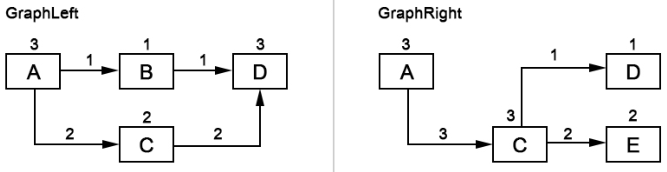
\includegraphics[width=0.8\textwidth]{Images/ProcessModels.PNG}
	\caption{Two process models.}
	\label{fig:ProcessModels}
\end{figure}

For generating the difference graph two process models are needed. These models can be described in many different process modeling languages eg. Petri Nets, BPMN, EPC. All of those languages which are conform to the above mentioned process model description can be used for the difference graph calculation. From both input process models the difference graph model is calculated. This model extends a process model with an element called marking. The marking is applied on edges and nodes and is generated during the calculation process.

%Noch auf die Unterschiede eingehen? ein Difference Model kann bsp. mehr wie einen start/endknoten haben

For calculating the markings the first model is subtracted from the second one. During the calculation three or five different markings can be generated. Five markings can be calculated if the input process models consist of weights. If not, only three markings can be calculated. The following list shows all five markings and gives a description in which case they are used. 

\begin{itemize}
	\item \textbf{New}, a node/edge gains the marking New when the node/edge was added from Input1 to Input2.
	\item \textbf{Positively changed}
	\item \textbf{Unchanged}, a node/edge gains this marking when its value matches in both inputs.
	\item \textbf{Negatively changed}
	\item \textbf{Deleted}
\end{itemize}

Hint the markings Positively changed and Negatively changed can not be calculated if the input process models do not consist weights.

Figure \ref{fig:DiffGraphCalculation} shows the results for subtracting Input2 from Input1 (Figure \ref{fig:ProcessModels}). Node B  was deleted from Input2 therefore, the marking deleted is applied the weight is calculated by subtracting 1 from 0 = -1. Node C was changed positively the weight has increased from 2 to 3.

\begin{figure}
	\centering
	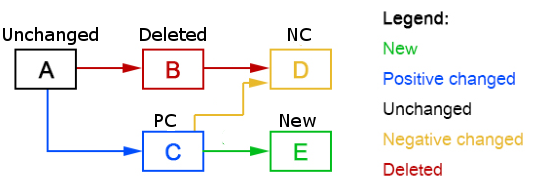
\includegraphics[width=0.8\textwidth]{Images/ResultGraph.PNG}
	\caption{Calculating the differences from Figure \ref{fig:ProcessModels} leads to this difference model. On top of each edge and node calculated weights and applied markings are shown. TODO: change colors to black, Add weights, adapt the legend.
	%TODO: change all colors to Black and state on top of each node and edge which marking is applied. This will lead to the following: first the reader sees the two inputs, then he/she sees the calculation and later on in the evaluation he/she sees how this markings which are stated here with text are visualized.
	}
	\label{fig:DiffGraphCalculation}
\end{figure}

The main  focus of this paper is how to visualize the difference graph. The idea behind the visualization of the difference model is to represent each of the markings with different styles. For example, each marking can be mapped to represent a specific symbol. This symbol can then be visualized on nodes and edges.

A survey was conducted to secure a good understanding of the difference graph visualization. To do so a literature research with the goal to find different visualization approaches was executed. Our first step was to find relevant keywords addressing the topic of difference visualization where collected and used within search engines. This led to a wealth of papers which where used as a basis for snowballing method where on one side other relevant papers where collected and on the other side new keywords where extracted. From the collected papers nine visualization approaches where extracted.

This section gave an overview about the fundamental process model which is the base for the difference graph model. We also showed how the difference graph model is calculated and which markings can be expressed on edges and nodes. For visualizing the model an appropriate style for markings has to be found which will be part of the next section.

\section{Evaluation} %  [5 Pages]
\label{sec:Evaluation} % [1/2 Page]
To address the research question, stated in Section 1, an online survey was conducted. Traditional ways like literature research and aggregation of information did not lead to an answer to our research question. However, we used the information found with literature research as input for our survey. The survey should show from the nine styles we found which of them fits the difference graph visualization best.


\subsection{Design} % [1/2 Page]
\label{sec:Design}
To avoid massive scrolling and simplify navigation through the survey it is divided into single pages. Single pages also come with the advantage that on each commit of a page we are able to validate the answers and give hints to the user where answers are missing. Overall the survey is divided into three groups introduction, styles and advanced/demographic questions.

The introduction gives an example how the difference graph is calculated and ask the user a question specific to this example. This question allows to check if the user understood the example or not. Further questions on the introduction page check the attendees knowledge about graphs.

Following the introduction are the styles for visualizing the difference graph. Each style is presented on a single page and consists of two main questions. A question to rate the expressiveness of the style and a question to assign markings to each node and edge. Assigning markings to nodes and edges will allow to check for intuitive understanding of the style.

In the advanced/demographic section we first ask the attendee to rank the styles according to their expressiveness. Ranking the styles after seeing all of them allows additional evaluations. Additional questions from this section are, for example, if edges and nodes should be represented with the same style or if the style of the difference graph should be determined by the size of the graph. The survey concludes with demographic questions e.g. age, gender, employment.


\subsection{Procedure} % [1/2 Page]
\label{sec:Procedure}
After finalizing the surveys design a two-sided pretest was conducted.

In the first pretest a discussion with two people took place where the overall question and answer wording was adapted to support the users understanding.

In our second pretest five people had to complete the survey and give advices what should be changed. During their survey they where encouraged to think loud and ask questions.  



Following the pretest, the actual survey was started by 73 participants from which 31 where completed.

\subsection{Results} % [3 Page2]
\label{sec:Results}

The results should focus on the styles,



\begin{figure}
	\centering
	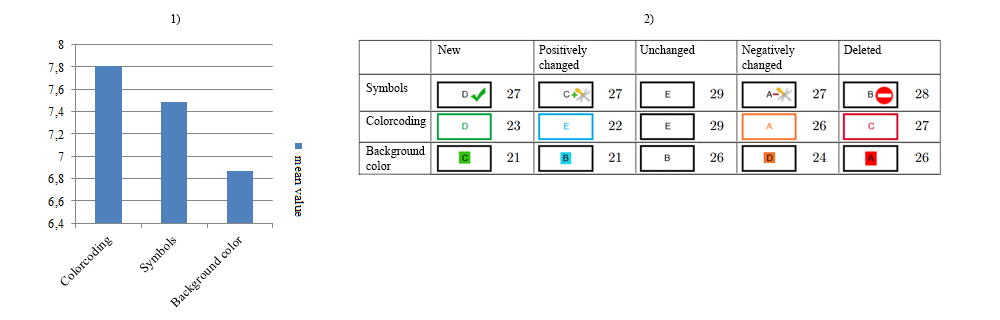
\includegraphics[width=1\textwidth]{Images/Results.PNG}
	\caption{SurveyResults}
	\label{fig:SurveyResults}
\end{figure}

Other results which should be shown are:
Understood the introduction? (answered the question correctly)
if edges and nodes should be represented with the same style?


Diff. Evaluations:
Intuitive understanding
Ranking



Summary:
Why we think color-Coding should be used.

\begin{figure}
	\centering
	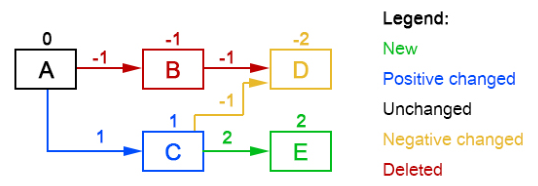
\includegraphics[width=0.8\textwidth]{Images/ColorCodedGraph.PNG}
	\caption{Final Representation of the Differencegraph}
	\label{fig:DiffGraphVisualization}
\end{figure}

\section{Applications}  % [1/2 Pages]
\label{sec:Applications}

Merging of processes -> Before merging two processes seeing where they differ from each other can be really good and support the merge process. For example activities which are only executed in one of the processes can be obtained easily.

Comparing two instances -> For example two factories which produce by same input the same output. Are there differences in process execution?

Evolution of a process -> Compare year 2013 and 2014, what has changed?


\section{Related Work}  % [1/2 Page]
\label{sec:RelatedWork}

Difference between the differencegraph concept and conformance checking?

Visual analytics


\section{Conclusion} %  [1/2 Page]
\label{sec:Conclusion}


\bibliography{Literature}
\bibliographystyle{plain}

\end{document}
